% ----- Consignes exo 1 ----- %
\begin{td-exo}[] % 1

\end{td-exo}

% ----- Solutions exo 1 ----- %
\iftoggle{showsolutions}{
	\begin{td-sol}[]\ % 1
		
	\end{td-sol}
}{}


% ----- Consignes exo 2 ----- %
\begin{td-exo}[] % 2

\end{td-exo}

% ----- Solutions exo 2 ----- %
\iftoggle{showsolutions}{
	\begin{td-sol}[]\ % 2
		On peut modéliser le problème comme suit:

        \ffigbox[\FBwidth]{%
\label{Fig:td1ex1c1}
}{
    \fbox{
        \begin{tikzpicture}[scale=1, every node/.style={circle, draw, fill=blue!20, inner sep=1pt, font=\scriptsize, minimum size=4mm}]
            \node (x1) at (0,0) {\(X_1\)};
            \node (x2) at (2,0) {\(X_2\)};
            \node (x3) at (4,0) {\(X_3\)};


            \node at (0,-1) {\(\scriptstyle 0\)};
            \node at (0,-2) {\(\scriptstyle 1\)};

            \node at (2,-1) {\(\scriptstyle 0\)};
            \node at (2,-2) {\(\scriptstyle 1\)};

            \node at (4,-1) {\(\scriptstyle 0\)};
            \node at (4,-2) {\(\scriptstyle 1\)};
            \node at (4,-3) {\(\scriptstyle 2\)};

            \draw (x1) -- (x2) node[midway, above] {\(\overset{4}{<}\)};
            \draw (x2) -- (x3) node[midway, above] {\(\overset{4}{<}\)};
            
        \end{tikzpicture}
    }
}

        On a 
        \begin{equation*}
            \forall x\in X, \forall c
        \end{equation*}
        %que porte son x?
        \(\forall x\in D(x),\exists t\) un tuple support solide
        pour tout \(x\) dans \(C\). Or 
        la valeur 1 de la variable \(X_1\) n'a pas de tuple support solide
        dans \(C\).

        Autre justification, la valeur 0 de la variable \(X_2\)
        n'a pas de tuple support solide dans \(C\).

        Pour la fermeture arc consistante:

        \begin{equation*}
            \left(
                X = \left\{
                    X_1,X_2,X_3
                \right\},
                D_{AC}(X_1)=\{0\},
                D_{AC}(X_2)=\{2\},
                D_{AC}(X_3)=\{1\},
                C = \left\{
                    c_1,c_2
                    \right\}
            \right)
        \end{equation*}
	\end{td-sol}
}{}


% % ----- Consignes exo xx ----- %
% \begin{td-exo}[] % xx

% \end{td-exo}

% % ----- Solutions exo xx ----- %
% \iftoggle{showsolutions}{
% 	\begin{td-sol}[]\ % xx
		
% 	\end{td-sol}
% }{}
